\documentclass{mscLiterature}
%
%
% Thesis data
%\mscDepartment{Delft Center for Systems and Control (\textsmaller{DCSC})}%
\mscProgram{Systems and Control}
%Change if needed to
%\mscProgram{Mechanical Engineering}
\mscFaculty{Mechanical, Maritime and Materials Engineering (3mE)}%
\mscName{E. B. Legrand}%
\mscDate{\today}%
\mscTitle{Towards a consistent interpretation of financial instruments in economic engineering using
          Noether's theorem.}%
\mscSubTitle{}%
\mscKeyWords{thesis, msc, subject}% only used in PDF properties
%\mscCoverPicture{STYLESTUFF/escher-2}% to place a picture ( here the example COVER.eps) on the back of the cover page
%
%
% Third party options (create text/logo on the copywrite page)
\mscThirdPartyText{The work in this thesis was supported by Rabobank. Their cooperation is hereby gratefully acknowledged.}
\mscThirdPartyLogo{STYLESTUFF/RABO_LOGO}
% NOTE: on the title page only the TU Delft logo is permitted.
%
%
%
% Finalize the thesis data
\setThesisInfo
%
% Use \includeonly{} to build only certain parts of your thesis
%\includeonly{introduction, real_chapter, empty_chapter, long_chapter}%
%
%PH Toegevoegd 24-10-2011
%allow (matlab) listing max 1pt flexibility between lines
\lstset{lineskip=0pt plus 1pt minus 0pt}

%% -------------------------------------------------------------------

%      _______   _____ ______   ___  _______   ___                        
%     |\  ___ \ |\   _ \  _   \|\  \|\  ___ \ |\  \                       
%     \ \   __/|\ \  \\\__\ \  \ \  \ \   __/|\ \  \                      
%      \ \  \_|/_\ \  \\|__| \  \ \  \ \  \_|/_\ \  \                     
%       \ \  \_|\ \ \  \    \ \  \ \  \ \  \_|\ \ \  \____                
%        \ \_______\ \__\    \ \__\ \__\ \_______\ \_______\              
%         \|_______|\|__|     \|__|\|__|\|_______|\|_______|              
%                                                                         
%                                                                         
%                                                                         
%  ________  ________  _________  ___  ________  ________   ________      
% |\   __  \|\   __  \|\___   ___\\  \|\   __  \|\   ___  \|\   ____\     
% \ \  \|\  \ \  \|\  \|___ \  \_\ \  \ \  \|\  \ \  \\ \  \ \  \___|_    
%  \ \  \\\  \ \   ____\   \ \  \ \ \  \ \  \\\  \ \  \\ \  \ \_____  \   
%   \ \  \\\  \ \  \___|    \ \  \ \ \  \ \  \\\  \ \  \\ \  \|____|\  \  
%    \ \_______\ \__\        \ \__\ \ \__\ \_______\ \__\\ \__\____\_\  \ 
%     \|_______|\|__|         \|__|  \|__|\|_______|\|__| \|__|\_________\
%                                                             \|_________|
%                                                                         

% --------------------------------------------------------------------
%% CUSTOM PACKAGES
% --------------------------------------------------------------------
\usepackage{cleveref}
\usepackage{siunitx}
\usepackage[official]{eurosym}
\usepackage{xspace}
\usepackage{physics}
\usepackage{tikz}
\usepackage{pgfplots}

% --------------------------------------------------------------------
%% COLORS
% --------------------------------------------------------------------

\definecolor{accent1}{RGB}{61,152,222}
\definecolor{accent2}{RGB}{216,74,59}
\definecolor{accent3}{RGB}{46,204,113}
\definecolor{accent4}{RGB}{241,196,15}
% \definecolor{gray_custom}{}{}

% TUD COLORS
% ----------------------------------

\definecolor{tudCyan}{RGB}{61,152,222}
\definecolor{tudBlack}{RGB}{0,0,0}
\definecolor{tudWhite}{RGB}{255,255,255}

% Basic colors
\definecolor{tudSeaGreen}{RGB}{111,189,165}
\definecolor{tudGreen}{RGB}{39,131,142}
\definecolor{tudDarkBlue}{RGB}{34,70,122}
\definecolor{tudPurple}{RGB}{36,46,131}
\definecolor{tudTurquoise}{RGB}{50,154,179}
\definecolor{tudSkyBlue}{RGB}{130,187,206}

% Accent colors
\definecolor{tudLavender}{RGB}{121,150,180}
\definecolor{tudOrange}{RGB}{216,130,62}
\definecolor{tudWarmPurple}{RGB}{110,50,122}
\definecolor{tudFuchsia}{RGB}{178,72,146}
\definecolor{tudBrightGreen}{RGB}{183,200,34}
\definecolor{tudYellow}{RGB}{247,234,151}

\definecolor{customBlockColor}{RGB}{200,228,250}
\definecolor{customAlertColor}{RGB}{31,112,173}

% --------------------------------------------------------------------
%% CUSTOM OPTIONS
% --------------------------------------------------------------------

\theoremstyle{definition}
\newtheorem{definition}{Definition}[section]

% SiUnitx

\DeclareSIUnit\money{\$}
\DeclareSIUnit\year{yr}

% --------------------------------------------------------------------
%% MATH MACRO's
% --------------------------------------------------------------------
\newcommand{\han}{\ensuremath{\xi}\xspace} % Hyperbolic angle
\newcommand{\hanv}{\ensuremath{\rho}\xspace} % Hyperbolic angular velocity
\newcommand{\amnt}{\ensuremath{A}\xspace} % Amount function
\newcommand{\ininv}{\ensuremath{K}\xspace} % Initial investment; arm
\renewcommand{\real}{\ensuremath{\mathbb{R}}\xspace}


% TikZ externalization - must be in main file!
\tikzexternalize[prefix=media/cache/]

\begin{document}
%
%========================== Front matter ======================================
\frontmatter %
%
% Make the cover page and hell of a lot of title pages
\maketitle
%
%
% Abstract (does not appear in the Table of Contents)
\chapter*{Abstract}%

\lipsum[1]

%
% table of contents, (\toc of \toclof of \tocloflot )
\tocloflot
%
%
%%
% Preface
\chapter{Preface}

\lipsum[1-2]
%%
% Acknowledgements
\chapter{Acknowledgements}%

I would like to thank my supervisor \mscreaderone\ for his assistance during the writing of this thesis\ldots

By the way, it might make sense to combine the Preface and the Acknowledgements.  This is just a matter of taste, of course.

\vspace*{15mm}

Delft, University of Technology \hfill \mscname \\
\mscdate
%%
% Dedication page. 
\cleardoublepage
\thispagestyle{empty}
\vspace*{\stretch{1}}

% Put your own motto here, or dedicate your work to your Mom or whatever...
\begin{quote}
\noindent``In the future, airplanes will be flown by a dog and a pilot. And the dog's job will be to make sure that if the pilot tries to touch any of the buttons, the dog bites him.''
	
--- \emph{Scott Adams}
\end{quote}

\vspace{\stretch{3}}
\clearemptydoublepage
%
%========================== Main matter ======================================
\mainmatter

%\subsection*{Structure literature study}
\begin{enumerate}
    \item Introduction
    \item Basic financial concepts
    \item Connection between finance and Lorentz plane 
    \begin{enumerate}
        \item Discounting, net present value, IRR, bond valuation etc.
        \item Matrix representation
        \item Discrete idea
        \item Connection discrete - continuous with `sampling time'
        \item Interest equation
    \end{enumerate}
    \item Hyperbolic numbers
    \begin{enumerate}
        \item Intro + literature
        \item Generalized complex numbers
        \item Definitions + operations
        \item Parameterizations
        \item Group structure
        \item Calculus
    \end{enumerate}
    \item Geometric Algebra (?) $\to$ no research performed yet
    \item Connection with special relativity
    \item Hyperbolic geometry
    \begin{enumerate}
        \item definition of hyperbolic spaces
        \item models of hyperbolic spaces
        \item basic properties
    \end{enumerate}
    \item Analytical mechanics
    \begin{enumerate}
        \item Lagrangian mechanics
        \item Hamiltonian mechanics
    \end{enumerate}
    \item Economic Engineering principles
    \begin{enumerate}
        \item Newtonian
        \item Energy-based
    \end{enumerate}
    \item Proposal for mechanical analogy
\end{enumerate}
% \chapter{Weekly questions}

\section*{Week 10: A First Entry into Special Relativity}

\begin{question}
    How does the hyperboloid model work exactly, and what does it look like in Euclidean and Minkowski space?
\end{question}

\emph{Minkowski space(time)} is a combination of a three-dimensional Euclidean space and time into a four-dimensional manifold\footnote{\url{https://en.wikipedia.org/wiki/Minkowski_space}}. The isometry group of Minkowski space is the Poincaré group (or the Lorentz group, in a slightly more specific fashion). The isometry group of a metric space is the group of transformations under the action of which the metric remains invariant. The Minkowski space is endowed with an indefinite nondegenerate bilinear form called the Minkowski metric (or inner product) which yields the spacetime interval. This metric is \textbf{not} Riemannian as it is not positive-definite but only nondegenerate, which is why the Minkowski space is categorized as a pseudo-Riemannian manifold. This simply means that the Minkowski metric might vanish for nonzero vectors.

The \textit{Minkowski quadratic form} is defined as \footnote{\url{https://en.wikipedia.org/wiki/Hyperboloid_model}}
$$ Q(x_0, x_1, \ldots, x_n) = x_0^2 - x_1^2 - \ldots - x_n^2 $$
The polarization (a way of expressing an inner product in terms of a norm) of the Minkowski quadratic form is the Minkowski bilinear form $B$
$$ B(\vb{u}, \vb{v}) = \frac{1}{2} (Q(\vb{u} + \vb{v}) - Q(\vb{u}) - Q(\vb{v}))$$
The space $\real^{n+1}$ endowed with the Minkowski bilinear form is precisely the aforementioned Minkowski (pseudo-Riemannian) space. The choice of this specific bilinear form sets it apart from the traditional Euclidean space of dimension $n+1$ ($\mathbb{E}^{n+1}$) --- they are the \emph{same manifold} equipped with a \emph{different metric}.

All vectors $\vb{v}\in \real^{n+1}$ such that $Q(\vb{v}) = 1$ form an $n$-dimensional hyperboloid $S$ connecting of two sheets (the `future' sheet $S^{+} = \{\vb{v} \in S \mid v_0 > 0\}$ and the `past' sheet $S^{-} = \{\vb{v} \in S \mid v_0 < 0\}$ ). The hyperboloid model only considers the points on future sheet. A straight line in hyperbolic $n$-space is modeled as a geodesic on the hyperboloid. 

\begin{framed}
It is important to bear in mind the distinction between the Minkowski space and the hyperbolic space. Minkowski space is a flat space endowed with the Minkowksi metric. Hyperbolic space is a curved space.
\end{framed}

A \emph{Hyperbolic space} is a space with constant negative curvature.

The Lorentz group preserves the hyperboloid in Minkowski space.

\begin{question}
    How does the Special Relativity concept `interval' work in in finance?
\end{question}
The interval in Special Relativity is equal to the initial amount invested. Under Lorentzian transformations, the spacetime interval is conserved.

\begin{question}
    How do Lorentz transformations work in finance?
\end{question}
In general, Lorentz transformations are either boosts or rotations. In finance, boosts represent the action of compounding interest, or a `time march'. There is a very important difference that has to be kept in mind: in the `finance' Lorentzian space there is no time axis: the `special' dimension is reserved for capital instead. As a result, the boost operation has a time-varying argument.

\begin{question}
    How does the Minkowski metric arise from a simple compounding process?
\end{question}
\Cref{fig:compounding_example} exemplifies the compounding process with 5\% interest on an initial investment of \si{\money}1000. For now, it is immaterial what the compounding frequency is. The total value of the investment is decomposed into two parts, which will be called the `capital' and `yield' fractions. Every time the investment is `compounded', the following happens:
\begin{itemize}
    \item The interest rate acts on the amount of capital outstanding, the result of which adds to the current total yield.
    \item The interest rate acts on the current total yield, the result of which is added to the capital outstanding. This is sometimes called \textit{interest on interest} and lies at the very core of the compounding principle. If this action would not be present, the process reduces to simple interest.
\end{itemize}
Clearly, apart from the obvious symmetry, this decomposition is motivated by its intuitive interpretability. Much of what is to come in the dissertation hinges on this principle, which is why this example, obvious as it may seem, is important. 
\begin{figure}[ht!]
    \centering
    \begin{tikzpicture}
        \path (-2, 1)  node[fill=white, align=center]     {\textbf{Invested capital}};
        \path (2, 1)   node[fill=white, align=center]     {\textbf{Yield}};
        \path (-2, 0)  node[fill=white, align=center](x1) {1000};
        \path (2, 0)   node[fill=white, align=center](y1) {0};
        \path (-2, -2) node[fill=white, align=center](x2) {$1000 + 0$};
        \path (2, -2)  node[fill=white, align=center](y2) {$0 + 50$};
        \path (-2, -4) node[fill=white, align=center](x3) {$1000 + 2.5$};
        \path (2, -4)  node[fill=white, align=center](y3) {$50 + 50$};
        \path (-2, -6) node[fill=white, align=center](x4) {$1002.5 + 5$};
        \path (2, -6)  node[fill=white, align=center](y4) {$100 + 50.125$};
        \path (-2, -8) node[fill=white, align=center](x5) {$1007.5 + 7.50625$};
        \path (2, -8)  node[fill=white, align=center](y5) {$150.125 + 50.375$};
        
        \draw[->] (x1) -- (x2);
        \draw[->] (x2) -- (x3);
        \draw[->] (x3) -- (x4);
        \draw[->] (x4) -- (x5);
        
        \draw[->] (y1) -- (y2);
        \draw[->] (y2) -- (y3);
        \draw[->] (y3) -- (y4);
        \draw[->] (y4) -- (y5);
        
        \draw[->] (x1) -- node[near start, sloped, above] {\footnotesize{$_{5\%}$}} (y2);
        \draw[->] (x2) -- node[near start, sloped, above] {\footnotesize{$_{5\%}$}} (y3);
        \draw[->] (x3) -- node[near start, sloped, above] {\footnotesize{$_{5\%}$}} (y4);
        \draw[->] (x4) -- node[near start, sloped, above] {\footnotesize{$_{5\%}$}} (y5);
        \draw[->] (y1) -- node[near start, sloped, above] {\footnotesize{$_{5\%}$}} (x2);
        \draw[->] (y2) -- node[near start, sloped, above] {\footnotesize{$_{5\%}$}} (x3);
        \draw[->] (y3) -- node[near start, sloped, above] {\footnotesize{$_{5\%}$}} (x4);
        \draw[->] (y4) -- node[near start, sloped, above] {\footnotesize{$_{5\%}$}} (x5);
    \end{tikzpicture}
    \caption{Caption}
    \label{fig:compounding_example}
\end{figure}
Two approaches will be discussed that elegantly capture this process from a computational standpoint:  discrete LTI systems and hyperbolic-complex numbers. These methods are also closely related and essentially represent two sides of the same coin. The results that follow should therefore not come as surprising, though looking at them from different perspectives is certainly instructive.

\subsubsection*{Split-complex numbers}

[...]

\subsubsection*{Discrete dynamic system}
The translation from the process displayed in \cref{fig:compounding_example} is fairly obvious:
$$ 
    \vb{x}(k+1) = \mqty(1& \hanv \\ \hanv & 1)\vb{x}(k)\qq{with }\vb{x}(0) = \mqty(\ininv\\0)
$$
The solution of this autonomous system is given by:
$$
    \vb{x}(k) = \mqty(1& \hanv \\ \hanv & 1)^k\mqty(\ininv\\0)
$$
In order to motivate the further usage of the Lorentzian $n$-space, one can evaluate the Lorentzian norm of $\vb{x}(k)$ as follows:
$$
    \vb{x}(k)\circ\vb{x}(k) = \mqty(K & 0)\mqty(1& \hanv \\ \hanv & 1)^k\mqty(1 & 0\\0 & -1)\mqty(1& \hanv \\ \hanv & 1)^k\mqty(K\\0)
$$
Using eigenvalue decomposition of the system matrix
$$
    \vb{x}(k)\circ\vb{x}(k) = \vb{x}(0)^\top V\Lambda^k V^{-1} M V^{-1} \Lambda^k V \vb{x}(0)
$$
with
$$
    V = \mqty(-1 & 1 \\ 1 & 1) \quad \Lambda = \mqty(1 - \hanv & 0\\0 & 1 + \hanv)\quad M = \mqty(1 & 0 \\ 0 & -1)
$$
Straightforward computations yield then
$$
    \vb{x}(k)\circ\vb{x}(k) = K^2\qty(1 - \hanv^2)^k
$$
Clearly, this suggests that the Lorentzian norm of $\vb{x}(k)$ is \emph{almost} equal to $K^2$ apart from the multiplication by a number slightly smaller than 1 for reasonably small values of $\omega$. At this point one must realize that a discrete compounding process is always an approximation to the ideal case, which is why the Lorentzian norm is not exactly invariant under the transformation of the system matrix. Instead, let's subdivide a single time step into multiple compounding steps to achieve a better approximation:
$$ \vb{x}\circ\vb{x} = K^2 \lim_{n\to \infty} \qty(1 - \qty(\frac{\hanv}{n})^2)^{nk}$$
The limit on the right can be shown to be equal to 1\footnote{cf. notes}, which means that for continuous compounding, the Lorentzian norm is conserved.

\subsubsection*{Continuous LTI model properties}


\begin{question}
    What is the difference between the Poincaré group and the Lorentz group?
\end{question}
Quick and dirty: Poincaré group = Lorentz group + spacetime translations

The Poincaré group is sometimes said to contain both homogeneous and inhomogeneous Lorentz transformation.

\section{Week 15: Explore Ideas from Max}

\begin{question}
    How can we map interest movements in the Lorentz plane to the Smith chart?
\end{question}
\emph{Max' idea}: Map the asymptotes to the circumference of a circle, the capital axis to the diameter. Question is therefore: which mapping do we need to accomplish this? 
The traditional mapping of the Smith chart is:
$$ \Gamma = \frac{B\exp{-2\gamma l}}{A\exp{+2\gamma l}}$$
with $A$, $B$ constants

The mapping to project the interest movements in the Smith chart is a product of two Möbius transforms: 
$$ f_1(z) = z^2 \quad f_2(z) = \frac{z + 1}{z - 1}\qquad f(z) = (f_2 \circ f_1 )(z)  = \qty(\frac{z + 1}{z - 1})\qty(\frac{z + i}{z -i})$$
the former map is the traditional Smith chart.

How does this translate to a matrix?

\begin{question}
    Extra dimension for investments.
\end{question}

% Introduction
\chapter{Introduction}
\label{chap:intro}
On the eight page of the October 16, 1929 edition of the New York Times, a small article headed \cite{NYT1929}
\begin{quote}
    \emph{``Fisher Sees Stocks Permanently High; Yale Economist Tells Purchasing Agents Increased Earnings Justify Rise."} 
\end{quote}
Responsible for this bold statement was Irving Fisher, a very prominent American economist who pioneered on the subject of monetary economics. Unfortunately for him, on Thursday the 29th of October --- merely nine days later --- the Dow Jones Industrial Average dropped by 11 percent, only to lower by another 13 percent on Monday, and then by 12 percent on Tuesday. The result was the Great Depression, an unprecendented financial crisis with dramatic repercussions: in the following three years, unemployment rose to 20 percent and industrial production almost halved \cite{gdepression}. 

Of course, this anecdote is not meant to discredit Irving Fischer as an economist, for he has been a major contributor to modern economic theory, but rather to illustrate that even specialists tend to misinterpret the current state of financial markets. This thesis does not aim to solve this issue right away, but to provide a new approach to the interpretation of the financial system; this may help in the understanding of this vital component of modern day society. This new approach is founded in the recent theoretic framework of economic engineering, developed by prof. em. M. Mendel \cite{Mendel2019}. 

\paragraph{Economic engineering} An introduction to relevant aspects of economic engineering will be provided in \cref{chap:ee}, but the core idea is to include economic systems in the traditional multi-domain modeling framework that (control) engineers use to study systems of widely varying nature (mechanical, electrical, hydraulic, etc.), possibly with the intention of develop a suitable control strategy. Of course, control strategies are vital for economic systems as well --- although this practice would probably be called `policy making' --- either on small scale, such as firms managing their stock levels and revenue in a changing market, or on macroeconomic scale, e.g. a central bank deciding whether to lower the interest rate or not.

Economic engineering research has been concerned with financial markets before: an economic analogy to the usage of 
\emph{action-angle coordinates} was exploited by \citet{Vos2019} to improve the models used for monetary policy. \citet{Kruimer2021} developed a macroeconomic model of the U.S. economy, where he included bond and equity markets as vital components of the economic machinery by means of the so-called \emph{rotational analogy}. Apart from the fact that both interpretations are manifestly different ways to describe the same concept, they appear to be flawed in some fundamental ways. As such, the necessity arises to reconcile these methods and address their problems in order to find a unifying economic engineering approach to incorporate financial systems; primarily concerning markets for equity and debt and perhaps their related derivatives such as futures and options. 

\paragraph{Current approach} As mentioned, economic engineering currently recognizes two ways to deal with 
`money problems'. Firstly, money is considered analogous to \emph{action}, as (will be explained in \cref{chap:ee}); action is a quantity that represents the integral of energy over time, with units [\si{\joule \second}]. Action-angle coordinates are a choice of coordinates in the phase space that consist of (constant) action coordinates and dimensionless `angles', indicating a \emph{periodic} motion. Secondly, there is the rotational analogy; which is arguably a bit more flexible than the action-angle coordinates. Again, based on dimensional analysis, an analogy can be made between `money' and angular momentum (in physics, angular momentum and action have the same dimension). Here the role of the angle represents a return or an accumulated interest, and `arm' of the rotation the principal of the investment/debt instrument.

\paragraph{Research goal} The core idea is that, instead of \emph{ad hoc} applying the existing theories, to return to the fundamentals of economic engineering and its ties with analytical mechanics to build a more rigorous foundation for future work. Energy and its analogy to utility in economics play a crucial role here, because (i) it lies at the foundation of analytical mechanics as well and (ii) it allows to make the connection with the existing (not strictly financial) theory of economic engineering, just like the multi-domain modeling techniques in engineering are connected through the universal concept of energy and power. Within analytical mechanics, Noether's theorem describes precisely how mathematical symmetries in the general nature of the system expressed in terms of energy (encoded in a special state function called the \emph{Lagrangian}) dictate \emph{conservation laws} that the system must obey. Naturally, perfect conservation of energy and momentum is equally unlikely in both physics and economics, but one strives nevertheless to construct a `platonic ideal', a conserved and isolated financial system to form the basis of the modeling framework.

The goal of this research can therefore be stated as follows: 
\begin{block}{Research goal}
    To develop a new, consistent, and unified framework to interpret debt and equity instruments in economic engineering, using the formal methods of analytical mechanics; and to provide an economic (or financial) interpretation to Noether's theorem.
\end{block}
\paragraph{Structure of the literature study} That being said, it is clear that the scope of this research is \emph{theoretical}, as its purpose is to expand and refine the current economic engineering framework. Hence, this literature study contains an overview of some related subjects that will hopefully play a role in the development of the theory. Firstly, in \cref{chap:ee} both the foundations of analytical mechanics and economic engineering are discussed in parallel; for each theoretical subject the fundamental analogies between both fields are emphasized for they form the cornerstones of this research. It is also in this chapter that Noether's theorem and the action-angle coordinates are introduced. Subsequently, \cref{chap:finance_rotation} provides a basic overview of finance and actuarial science; especially understanding the latter is vital to see why the rotational analogy works. Because the rotational analogy concerns a \emph{hyperbolic rotation} instead of a normal one, some additional 




% Second chapter
\chapter{Economic engineering}
Economic engineering is build on analogies between (macro)economic theory and common engineering disciplines such as thermodynamics, circuit theory and (classical) mechanics\footnote{as opposed to more recent theories in relativistic mechanics and quantum mechanics}. Escpecially for the latter, a rich variety of useful analogues can be devised. There are two common classses of interpretations mechanics: \emph{analytical mechanics} including the formulations by Joseph-Louis Lagrange and sir William Rowan Hamilton, and \emph{vectorial mechanics}, better known as \emph{Newtonian mechanics}. The former variant is usually preferred in the field of engineering whereas the analytical mechanics are due to their mathematical elegance powerful interpretative value. Likewise, the theory of economic engineering can be approached in two similar ways. Usually the `Newtonian' approach is given the most attention, but in the case of this work the energy-based approach will prove to be more useful, which is why it will be the starting point of this discussion instead.

\section{Analytical approach}
Analytical mechanics, more specifically \emph{Lagrangian} and \emph{Hamiltonian} mechanics, are built around the definition of special state functions, respectively called the Lagrangian \(\lag\) and the Hamiltonian \(\ham\).

\subsection{Lagrangian mechanics}
Central to the concept of Lagrangian mechanics is the so-called \emph{configuration space} \(M\), which is an \(n\)-dimensional manifold provided with some parameterization called \emph{generalized coordinates} assembled in the vector \(\vec{q}\). In classical mechanics, these generalized coordinates parameterize completely every allowable position of the system at issue. In economic engineering, \(\vec{q}\) has a similar intuitive notion, namely the stock values of various products, which denote the `position' of some economic system. Just as in mechanics, the configuration manifold may just be equal to \(\real^n\), but in more interesting and realistic cases it is often some manifold embedded in \(\real^n\). 

The Lagrangian \(\lag\) is then defined as a mapping from the \emph{tangent bundle} \(TM\) of the configuration manifold \(M\) , optionally paired with a time argument for time-varying problems to the reals,
    \[ \lag : TM \times \real^+ \to \real, \]
i.e. it takes a generalized position \(\vec{q}\) and a generalized velocity \(\dot{\vec{q}}\) (which live in the tangent space of \(M\)), and a time instance to some scalar value. The crux of the Lagrangian theory is that motions of a mechanical system coincide with \emph{extremals}\footnote{this is a natural extension of the term \emph{extremum} to the calculus of variations.} of the action integral
\[ \Phi(\gamma) = \int^{t_1}_{t_0} \lag \dd{t}\]
where by convention \(\lag = \mathscr{T}^{*} - \mathscr{V}\), i.e. the difference between the kinetic co-energy and potential energy in the system. In economic engineering, the lagrangian is analogous to running costs. Hence, the extremal of the aforementioned integral coincides with a cost minimization, which fits will into the rational behaviour of economic agents on whatever scale.

\begin{block}{Lagrangian system}
    Let \(M\) be a differentiable manifold, \(TM\) its tangent bundle, and \(\lag: TM \to \real\) a differentiable function. A map \(\gamma: \real \to M\)  is called a motion in the lagrangian system with configuration manifold \(M\) and lagrangian function \(\lag\) if \(\gamma\) is an extremal of the functional
    \[
     \Phi(\gamma) =  \int^{t_1}_{t_0} \lag\qty(\dot{\gamma})\dd{t}
\]
    where \(\dot{\gamma}\) is the velocity vector \(\dot{\gamma}(t) \in TM_{\gamma(t)}\) \cite{Arnold1989}.
\end{block}

\subsection{Hamiltonian mechanics}

\section{Newtonian approach}

\chapter{Investment as a hyperbolic rotation}
\label{chap:finance}

\section{The concept of interest}
Usually, two types of interest are distinguished: simple interest and compound interest. The key difference is that in the case of compound interest, the money earned (or due) on an interest-bearing instrument is subject to interest itself. That is, if somebody takes out a loan, the corresponding interest payments are also considered as a contribution to the principal and therefore result in higher future interest payments. In contrast, the case of simple interest does not consider the compounding effect; the interest payments remain constant over time. 

The compounding of interest is always associated with a certain period; this is the period over which the interest earned is calculated and added to the amount due (or `reinvested' in case of an investment). The choice of this period is part of the agreement between the lender and the borrower, common compounding periods are daily, weekly, monthly or yearly. From a mathematical perspective, one can view the choice of compounding period as a limiting process: clearly, the choice in practice is rather arbitrary. Indeed, the `ideal' compounding period is continuous, but before the advent of computers this was not achievable in practice; in banking applications it is still not very commonly used \cite{Zipf2003}.

\subsection{Interest terminology}
Many interest calculations are subject to conventions, which is why there are several terms associated `interest' which must be clearly distinguished. Usually, an interest-bearing instrument is associated with some amount that is initially borrowed or invested, which is called the \emph{principal}, denoted by \(K\). Secondly, one can define the \emph{accumulation function} \(a\) which yields the accumulated value of a unit investment (or loan).\footnote{In this discussion, the distinction between credit or debit (i.e. investments or loans) is quite irrelevant for the principles at hand, they just differ in sign on the balance sheet of the respective counterparties. Hence, these terms will be used interchangeably. Minus signs are there to indicate cash flows in the `opposite' direction, regardless whether this is on the credit or debit side of the balance sheet.}
Similarly, the \emph{amount function} \(A\) measures the accumulation of any principal value \(K\): \(A(k) = Ka(k)\). \cite{Kellison1991}

Concerning the period \(k\), some additional remarks are in order. In most banking applications, the interest process is discrete, i.e. the compounding effect occurs over discrete intervals. Apart from the compounding process, one can distinguish a `measurement' interval which can, but does not necessarily have to, coincide with the compounding period. For now, the interest process is assumed to be calculated on a discrete basis; the transition to continuous time will be made after that.

\begin{thmblock}{Effective rate of interest}
    The \emph{effective rate of interest} \(r\) is the ratio of the amount of interest earned during the period to the amount of principal invested at the beginning of the period. In terms of the accumulation function:
     \begin{equation}
         i(k) = \frac{a(k) - a(k-1)}{a(k-1)}
         \label{eq:effective_interest}
     \end{equation}
     where \(a\) is in this case assumed to take discrete values.
\end{thmblock}


\subsubsection{Simple interest}
For the case of simple interest, the accumulation function has the form
\[
     a(k) = ik + 1
\] 
where \(i = i(0)\) denotes the constant simple interest rate, which turns out to be identical to the effective rate of interest over the first period. An important fact one has to bear in mind is that for the case of simple interest the effective rate of interest is \emph{not} constant over time (this, in fact, motivates the existence of compound interest, as will become clear later). Using \cref{eq:effective_interest}:
\[
     i(k) = \frac{\qty(ki + 1) - \qty[(k-1)i + 1]}{(k-1)i + 1} = \frac{i}{1 + i(n-1)}
\]
which means that simple interest results in a decreasing effective rate of interest over time. \cite{Kellison1991}

\subsubsection{Compound interest}
As mentioned before, compound interest relies on the reinvestment of the interest already earned. At the end of the period the accumulation function is a factor \(1 + i\) larger than the period before. One can therefore say that
\[
     a(k) = (1 + i)a(k-1)\quad\text{or}\quad a(k) = (1 + i)^{k}
\]
assuming that the compounding period coincides with the measurement period. 

Similarly, \cref{eq:effective_interest} can be used to compute the effective rate of interest for an arbitrary period:
\[
     i(k) = \frac{(1 + i)^k - (1 + i)^{k-1}}{(1 + i)^{k-1}} = i
\]
which means that for compound interest, the effective rate of interest is \emph{constant}. This is the reason why compound interest plays an ubiquitous role in modern finance; otherwise it would become less and less profitable for investors to keep  their money in a certain investment (they would rather just stay a single period and then turn to a new investment --- this effectively emulates compound interest!). Only for short periods (less than one year), simple interest is sometimes used because the difference with compound interest is negligible, which can be motivated by means of the Taylor series of \(a\) for compound interest: 
\[
     (1 + i)^k = 1 + i +  \binom{k}{2}i^2 + \binom{k}{3}i^3 + \ldots \approx 1 + i\qfor i \ll 1,\ k \text{ small}
\]
In fact, from this equation it is clear that simple interest and compound interest yield the same result after the first compounding period, after which compound interest will take the upper hand.

For now, it was assumed that one compounding period is equal to one measurement period. However, this does not necessarily have to be the case. More generally, one can write the accumulation function as:
\[
     a(k) = \qty(1 + \frac{i}{n})^{nk}
\]
where \(n\) is the number of compounding periods per measurement periods (which is assumed to be an integer number). In actuarial sciences, the measurement period is normally equal to one year; meaning that e.g. weekly compounding amounts to \(n = 52\).

Here, \(i\) is called the \emph{nominal interest rate}, which is usually denoted by \(i^{(n)}\), indicating that the nominal rate \(i\) is compounded \(n\) times at a rate \(i^{(n)}/n\). Hence, a nominal interest rate of \(i^{(m)}\) per measurement period is equivalent to an effective interest rate of \( i^{(m)}\) per \(n\)th part of that measurement period. 

The effective rate of interest measures the relative growth of an investment over one compounding period. Although this may seem like an obvious definition, the very nature of the financial investments is encoded in it: the return of some investment is proportional to the amount invested originally, and because the earnings can be `converted' into capital again (because both are `money', this important step is often taken for granted), they can be reinvested. This is, as will become clear, the reason for the exponential growth of money. One should, however, be cautious to associate this process exclusively with financial investments; for example a farmer could use the earnings from his land to buy more land, increase his earnings, use those again to buy even more land and so forth --- this will again give rise to a exponential growth. The farming example makes it quite clear that the object that `generates' the return (capital) is of a very different nature than the return itself (yield). They can be connected through money, which makes the whole process work. 

Financial investments are arguably the culmination of this concept, since money itself earns money that can be reinvested again instantaneously. Still, the capital-yield distinction remains relevant: for example, companies pay dividends to their shareholders in proportion to the amount of stock they own; the shareholders could then choose to reinvest these earnings in more stock of that (or another) company, increasing their `capital'. Again, the distinction between capital and yield is clear, but may be obscured by the fact that both stocks and their dividends are expressed in terms of money\footnote{An additional example here are \emph{stock dividends}, which are stocks with dividends that are paid as additional stock --- essentially taking the role of money out of the equation.}. 

\subsubsection{Continuous time}
Now, the discrete accumulation (and amount) functions will be converted to their continuous counterparts, since that will be the most convenient form from a mathematical perspective. To do so, consider the nominal interest over single measurement period, but subdivided into an ever growing number of compounding intervals. Because the number of compounding intervals grows to infinity, the choice of measurement interval becomes immaterial which is why it can simply be replaced by `\(t\)' denoting continuous time.

In case of simple interest, the result is trivial:
 \[
     a(t) = \lim_{n \to +\infty} \qty(\frac{i}{n}) (tn) + 1 = it + t
\]
which basically means that the nominal interest remains the same no matter the `compounding period'.

For compound interest, the result is more interesting:\footnote{There exist a few equivalent definitions of the exponential function, one of which is this limit. As such, some may argue that this statement is true \emph{by definition}.}
 \[
     a(t) = \lim_{n \to \infty} \qty(1 + \frac{i}{n})^{nt} = \ec^{it}
\]
 
\subsection{Discounting, Net Present Value and the Internal Rate of Return}
\ac{IRR}
\ac{NPV}
\index{Net Present Value}
\index{Discounting}
\index{Internal Rate of Return}


\subsection{Lorentz structure from the compounding process}
\Cref{fig:compounding_example} exemplifies the compounding process with 5\% interest on an initial investment of \si{\money}1000. For now, it is immaterial what the compounding frequency is. The total value of the investment is decomposed into two parts, which will be called the `capital' and `yield' fractions. Every time the investment is `compounded', the following happens:
\begin{itemize}
    \item The interest rate acts on the amount of capital outstanding, the result of which adds to the current total yield.
    \item The interest rate acts on the current total yield, the result of which is added to the capital outstanding. This is sometimes called \textit{interest on interest} and lies at the very core of the compounding principle. If this action would not be present, the process reduces to simple interest.
\end{itemize}
Clearly, apart from the obvious symmetry, this decomposition is motivated by its intuitive interpretability. Much of what is to come in the dissertation hinges on this principle, which is why this example, obvious as it may seem, is important. 
\begin{figure}[ht!]
    \centering
    \begin{tikzpicture}
        \path (-2, 1)  node[fill=white, align=center]     {\textbf{Invested capital}};
        \path (2, 1)   node[fill=white, align=center]     {\textbf{Yield}};
        \path (-2, 0)  node[fill=white, align=center](x1) {1000};
        \path (2, 0)   node[fill=white, align=center](y1) {0};
        \path (-2, -2) node[fill=white, align=center](x2) {\(1000 + 0\)};
        \path (2, -2)  node[fill=white, align=center](y2) {\(0 + 50\)};
        \path (-2, -4) node[fill=white, align=center](x3) {\(1000 + 2.5\)};
        \path (2, -4)  node[fill=white, align=center](y3) {\(50 + 50\)};
        \path (-2, -6) node[fill=white, align=center](x4) {\(1002.5 + 5\)};
        \path (2, -6)  node[fill=white, align=center](y4) {\(100 + 50.125\)};
        \path (-2, -8) node[fill=white, align=center](x5) {\(1007.5 + 7.50625\)};
        \path (2, -8)  node[fill=white, align=center](y5) {\(150.125 + 50.375\)};
        
        \draw[->] (x1) -- (x2);
        \draw[->] (x2) -- (x3);
        \draw[->] (x3) -- (x4);
        \draw[->] (x4) -- (x5);
        
        \draw[->] (y1) -- (y2);
        \draw[->] (y2) -- (y3);
        \draw[->] (y3) -- (y4);
        \draw[->] (y4) -- (y5);
        
        \draw[->] (x1) -- node[near start, sloped, above] {\footnotesize{\(_{5\%}\)}} (y2);
        \draw[->] (x2) -- node[near start, sloped, above] {\footnotesize{\(_{5\%}\)}} (y3);
        \draw[->] (x3) -- node[near start, sloped, above] {\footnotesize{\(_{5\%}\)}} (y4);
        \draw[->] (x4) -- node[near start, sloped, above] {\footnotesize{\(_{5\%}\)}} (y5);
        \draw[->] (y1) -- node[near start, sloped, above] {\footnotesize{\(_{5\%}\)}} (x2);
        \draw[->] (y2) -- node[near start, sloped, above] {\footnotesize{\(_{5\%}\)}} (x3);
        \draw[->] (y3) -- node[near start, sloped, above] {\footnotesize{\(_{5\%}\)}} (x4);
        \draw[->] (y4) -- node[near start, sloped, above] {\footnotesize{\(_{5\%}\)}} (x5);
    \end{tikzpicture}
    \caption{Caption}
    \label{fig:compounding_example}
\end{figure}
Two approaches will be discussed that elegantly capture this process from a computational standpoint:  discrete LTI systems and hyperbolic-complex numbers. These methods are also closely related and essentially represent two sides of the same coin. The results that follow should therefore not come as surprising, though looking at them from different perspectives is certainly instructive.

\begin{figure}
    \centering
    \begin{tikzpicture}[scale=1]
    \begin{axis}[
        xlabel={Invested capital $X$},
        ylabel={Yield $Y$},
        grid,
        cycle list name= black white,
        legend pos = south east,
        ymin = 0,
    ]
        \addplot coordinates {
                    (1000   ,  0     )
                    (1000   ,  50     )
                    (1002.5,  100    )
                    (1007.5,  150.125)
                    (1015.01,  200.5 )
                    (1025.03,  251.25)
                    (1037.59,  302.502)
                    (1052.72,  354.382)
                    (1070.44,  407.018)
                    (1090.79,  460.539)
                    (1113.82,  515.079)
                    (1139.57,  570.77)
                    (1168.11,  627.748)
                    (1199.5,  686.154)
                    (1233.8,  746.128)
                    (1271.11,  807.818)
                    (1311.5,  871.374)
                    % (135.507,  93.6949)
                    % (140.192,  100.47)
                    % (145.215,  107.48)
        };
        \addlegendentry{Yearly comp.};
        
        \addplot coordinates {
            (1000., 0.0)
            (1001.2502604383691, 50.020835937655015)
            (1005.0041680558036, 100.16675001984403)
            (1011.2711095766704, 150.56313315161269)
            (1020.0667556190758, 201.336002541094)
            (1031.4130998795731, 252.6123168081683)
            (1045.3385141288605, 304.52029344714266)
            (1061.8778191559855, 357.18972943727195)
            (1081.0723718384547, 410.7523258028155)
            (1102.970168555971, 465.34201693419774)
            (1127.6259652063807, 521.0953054937474)
            (1155.101414123941, 578.1516037434543)
            (1185.4652182422679, 636.6535821482414)
            (1218.793302887456, 696.7475261264401)
            (1255.169005630943, 758.5837018395335)
            (1294.6832846768447, 822.3167319358299)
            (1337.4349463048446, 888.1059821876231)
            (1383.530891937359, 956.1159599886322)
            %(143.30863854487743, 102.65167257081754)
            %(148.62253413851738, 109.94843179306726)
            %(154.30806348152436, 117.52011936438014)
        };
        \addlegendentry{$x^2 - y^2 = 1000^2$};
        
    \end{axis}
\end{tikzpicture}

    \caption{blabla}
    \label{fig:my_label}
\end{figure}

\chapter{The Lorentz-Minkowski Plane}

\begin{framed}
    \textbf{Chapter structure}
    \begin{enumerate}
        \item Definition
        \item Hyperbolic numbers
        \item Connection with Special relativity
        \item Smith chart
    \end{enumerate}
\end{framed}

It has now been established that for continuous compounding can, from the right perspective, be viewed as a hyperbolic process. Of course, this is the as much the case for compound interest as for other exponential processes, such as radioactive decay, population growth, the spreading of disease etc. However, one might argue that in the case of compound interest, the analogy is particularly useful for a few reasons:
\begin{itemize}
    \item The decomposition into `capital' and `yield' has a direct financial interpretation.
    \item The complete hyperbola consists of two different `sheets': one positive and one negative. These two sheets can be interpreted as the difference between `debit' and `credit'.
\end{itemize}
One sheet (the positive one) of the hyperbola can be seen as a model of the one-dimensional hyperbolic space $\mathbb{H}^1$. More generally, the hyperbolic $n$-space can be seen as a circle with imaginary radius, i.e. $$\mathbb{H}^n = \qty{
x \in \mathbb{R}^{n+1},\ r \in \mathbb{R}^{+}_{*} : \norm{x}^2 = -r}$$. As such, hyperbolic spaces have a constant negative curvature.

\begin{figure}
    \centering
    \begin{tikzpicture}[scale=1.5]
        %\draw[step=0.5, gray, very thin] (-2, -2) grid (2, 2);
        \draw[->] (-2, 0) -- (2, 0) node[right] {$x$};
        \draw[->] (0, -2) -- (0, 2) node[anchor=south] {$y$};
        \draw[domain=0:1.3, variable=\t, thick, red] plot ({cosh(\t)}, {sinh(\t)}) node[anchor=south] {Debit + interest};
        \draw[domain=-1.3:0, variable=\t, thick, red!50] plot ({cosh(\t)}, {sinh(\t)});
        \draw[domain=0:1.3, variable=\t, thick, tudCyan, thick] plot ({-cosh(\t)}, {-sinh(\t)}) node[anchor=north] {Credit + interest};
        \draw[domain=-1.3:0, variable=\t, thick, tudCyan!50] plot ({-cosh(\t)}, {-sinh(\t)});
        \node[tudCyan!50] at (-2, 2) {Credit + discount};
        \node[red!50] at (2, -2) {Debit + discount};
        \node[draw] at (0, 2.7) {$x^2 - y^2 = K^2$};
    \end{tikzpicture}
    \label{fig:credit_debit}
    \caption{Different parts of the complete hyperbola $x^2  - y^2 = K$ each have their distinct financial interpretation.}
\end{figure}
\chapter{Hyperbolic geometry}
\chapter{Möbius transforms}
\label{chap:moebius_transforms}
\index{Möbius transformation}

\section{Definition and basic properties}
Many of the transforms and mappings discussed in the preceding chapters may be expressed as a Möbius transformation. These are mappings of the form \cite{Needham1997}
\begin{equation}
    \mathfrak{M}(z) = \frac{az + b}{cz + d}
    \label{eq:mobius}
\end{equation}
where \(a, b, c, d \in \complex \) are constants. Möbius transformations carry a deep connection with hyperbolic geometry (and non-Euclidean in general), and Einsteins theory of relativity. As such, the connection with the financial interpretation of the Lorentz plane can be readily made. As stated by \citet{Needham1997}, the complex mappings that correspond to a Lorentz transformation are Möbius transformations and vice versa --- every Möbius transform corresponds to a unique Lorentz transformation.

The Möbius transformation \(\mathfrak{M}\) is called \emph{singular} if \(ad - bc = 0\), which maps every point to the same image \(a/c\). In general, any Möbius transformation can be decomposed into four elementary transformations:
\begin{enumerate}
    \item A translation \(z \mapsto z + \frac{d}{c}\)
    \item A \emph{complex inversion} \(z \mapsto \frac{1}{z}\)
    \item An expansion and rotation \(z \mapsto -\frac{ad - bc}{c^2}z\)
    \item A translation \(z + \frac{a}{c}\)
\end{enumerate}
Each of these transformations are conformal and preserve circles which is why general Möbius transformations inherit these vital properties as well. 

It is quite clear from \cref{eq:mobius} that multiplication of both the denominator and the numerator by the same constant \(k\) will not affect the result of the mapping. Therefore, a Möbius transformation is uniquely determined by only three quantities \(a/b, b/c\) and \(c/d\). This ambiguity allows for the notion of \emph{normalized transformations}, for which \(ad - bc = 1\). 

If \(\mathfrak{M}\) is nonsingular, the transformation is bijective; the inverse transformation is then given by \cite{Needham1997}
\[ \mathfrak{M}^{-1}(z) = \frac{dz - b}{-cz + a} \]

\section{Group structure}
It is neither surprising nor hard to show that the nonsingular Möbius transformations form a group under composition; the identity mapping is a Möbius transformation, the inverse transformation is also a Möbius transformation as illustrated by the expression for \(\mathfrak{M}^{-1}\) stated above and that the composition of two transformations \(\mathfrak{M}_2 \circ \mathfrak{M}_1\) again yields a member of the class of Möbius transformations \cite{Needham1997}. 

\subsection{The Riemann sphere}
The Möbius group \moebiusgroup is the automorphism group of the Riemann sphere. Being the simplest compact Riemann surface, the Riemann sphere is a special representation of the extended complex plane\footnote{The complex plane combined with a value for infinity `\(\infty\)'.} \(\hat{\complex}\) in three-dimensional space: it can be visualized by placing the complex plane horizontally and considering a unit sphere centered around the origin, such that its intersection coincides with the unit disk of the complex plane. To map the plane to the sphere, a stereographic projection is is used from the `north pole' of the sphere. As such, anything inside the unit disk is mapped to the southern hemisphere, everything on the unit disk is mapped onto itself (since it lies at the intersection) and everything outside the unit disk lies on the northern hemisphere. The north pole of the Riemann sphere then coincides with the distinctive feature of the extended complex plane, namely the point at infinity \(\infty\) \cite{Needham1997}. Stated more formally:
\[ \moebiusgroup = \automorphgroup{\hat{\complex}} \quad \hat{\complex} = \complex \cup \{\infty\}.\]
\index{automorphism group}
\index{Riemann sphere}
\index{extended complex plane}

In order to turn towards the computational aspect of the Riemann sphere, one must consider a different coordinate system for the complex plane; namely the \emph{homogeneous} or \emph{projective} coordinates. These consist of an ordered pair of complex numbers\footnote{In physics, these objects are also called \emph{2-spinors} which are also fundamentally connected with the theory of relativity, as demonstrated by \cite{Penrose1984}.} , i.e. an element of \(\complex^2/\left\{[0, 0]\right\}\),  denoted as \(\qty[\mathfrak{z}_1, \mathfrak{z}_2]\). These two complex numbers are subject to an equivalence relation that makes them projective coordinates, in that \[\qty[\mathfrak{z}_1, \mathfrak{z}_2] \sim \qty[\mathfrak{w}_1, \mathfrak{w}_2] \iff \mathfrak{w}_1 = \lambda \mathfrak{z}_1 \text{ and } \mathfrak{w_2} = \lambda \mathfrak{z}_2\]
with \(\lambda\) any nonzero complex number. The projective space is then formed by the quotient set of the complex 2-space (excluding the origin) and this equivalence relation. Every equivalence class can be uniquely identified with a point \([1, \sfrac{\mathfrak{z}_2}{\mathfrak{z}_1}]\), which then corresponds to a point on the The Riemann sphere (or equivalently on the extended complex plane). The only point where this mapping breaks down is the point \([0, 1]\), which can be associated with the north pole on the Riemann sphere, or the infinity point. In technical terms, this is called a one-point compactification of a plane into a sphere, with the desirable property that the infinity point \emph{has no special meaning on the sphere}, which it inevitably has in a plane. The Riemann sphere is therefore equal to the one-dimensional complex projective space \(\mathbb{CP}^1\) \cite{Thurston1997}. 
\index{compactification}

\subsection{Matrix representation}
A very powerful property of Möbius transforms is that they can each be associated to a \(2\times 2\) complex matrix like so:
\[ \frac{az + b}{cz + d} \corresponds \mqty(a & b \\ c & d).\] 
Because the transformations are only defined up to multiplication of a constant, so is associated matrix. However, one can assume to have the transformation normalized, i.e. \(ad - bc = 1\) which is equivalent to restricting the matrix to have a unit determinant.  When normalized, there are precisely two matrices corresponding to every Möbius transform, since multiplying the entire matrix with -1 would still yield the same result. Now, how can one actually effect a Möbius transformation using this matrix representation? This is where the projective coordinates come into play. As it turns out, 
\[ 
    \mqty(a & b\\ c & d)\mqty(\mathfrak{z}_1\\\mathfrak{z}_2)
    = \mqty(a\mathfrak{z}_1 + b\mathfrak{z}_2\\c\mathfrak{z}_1 + d\mathfrak{z}_2)
    =\mqty(a(\mathfrak{z}_1/\mathfrak{z}_2) + b\\c(\mathfrak{z}_1/\mathfrak{z}_2) + d)
\]
which are exactly the homogeneous coordinates of the image of \(z\) under this Möbius transform. This allows to calculate the result of any Möbius transformation also by means of a matrix multiplication.

The correspondence with matrices goes even deeper than this simple computational trick: the composition of two Möbius transforms  can simply be obtained by multiplying their corresponding matrices (denoted by \(M_1\) and \(M_2\)), that is
\[\mathfrak{M}_1 \circ \mathfrak{M}_2 \to M_1 M_2,\]
and furthermore, the inverse Möbius transformation \(\mathfrak{M}^{-1}\) corresponds to the inverse of the matrix \(M^{-1}\) \cite{Needham2021}.

\index{Möbius group}
\index{homogeneous coordinates}
\index{projective coordinates}
\index{complex projective line}

\subsection{The Möbius group} 
The link with the matrices already hints at a very important fact about Möbius transforms: they form a group under composition --- the Möbius group \moebiusgroup. This fact is actually immediately clear from the correspondence between matrix multiplication and composition of the transformation: a composition of two transforms is again a transform. Additionally, matrix multiplication is associative and they are assumed to be nonsingular, so inverses always exist. As such, all the group axioms are satisfied (of course, all these results could have been obtained directly from the definition of the Möbius transform, but the reasoning based on the matrices is particularly straightforward). Perhaps not very suprising is that the identity Möbius transformation \(E(z)\) corresponds to the \(2\times 2\) identity matrix.

Based on the matrix analogy, the one can state that \moebiusgroup is the group of linear\footnote{It is misleading to call the Möbius transforms `linear' in general --- they are definitely nonlinear in the complex plane! However, when using the homogeneous coordinates, they become linear transforms.} tranformations on vector space \(\complex^2\) --- as projective coordinates. This is the same as saying that the Möbius group is isomorphic to the group of linear transformations \emph{modulo} the nonzero scaling operation on \(\complex^2\): the resulting quotient group is the \emph{projective linear group} \pglgroup{2}{\complex}.

An interesting fact from group theory arises here as well: it has already been established that Möbius transforms are only unique up to multiplication by a scalar --- as such, they can be normalized (with unit determinant) without loss of generalization. This suggests that \moebiusgroup is really the action of the \emph{special} linear group modulo scalar multiplication, resulting in the \emph{projective special linear group}. Luckily, this fact is also reconciled within group theory: the groups \pglgroup{n}{\field} and \pslgroup{n}{\field} over the field \field are isomorphic as long as every element of \field has an \(n\)th root within \field. The fact that is is true for \(\field = \complex\) is probably the most fundamental property of the complex numbers. To summarize, the Möbius group \moebiusgroup is equal to the projective linear group and the special projective group (over the field of complex numbers), which are isomorphic to each other in this particular case.
\index{projective linear group}
\index{special projective linear group}

\section{Classification of Möbius transforms}
In the preceding discussion about the matrix representation of Möbius transforms, one important aspect has not yet been addressed: what about the eigenvalues and eigenvectors of \(M\)? Eigenvectors are vectors that remains invariant (up to scaling) under the multiplication of a particular matrix. Of course, one should bear in mind that the vector in this case contains projective coordinates, so that even when scaled, its coordinate representation remains identical. As such, the eigenvectors of the matrix \(M\) are the \emph{fixed points} of the Möbius transform \(\mathfrak{M}\); any Möbius transform has two at most. This is even more perspicuous by solving the equation \(z^* = \mathfrak{M}(z^*)\), which has solutions
\[ z^* = \frac{(a - d) \pm \sqrt{(a + d)^2 - 4}}{2c}.\]
When converted to projective coordinates, the two solutions for \(z^*\) then coincide with the eigenvectors of \(M\). In the degenerate case for which \(a + d = \pm2\), the argument of the square root amounts to zero, which means that there is only one unique fixed point. These transforms are called \emph{parabolic}, more will become clear about them later \cite{Needham1997}.

Now, it remains to analyse the significance of the eigenvalues. Of course, since eigenvalues are sensitive to scaling of the matrix, it is important to stress again that \(M\) must be normalized (have a unit determinant) in order for the following to hold. A well known fact in linear algebra states that if \(\lambda_1, \lambda_2\) are eigenvalues of \(M\), then
\[ \trace{M} = \lambda_1 + \lambda_2 \quad\text{and}\quad \det M  = \lambda_1 \lambda_2.\]
Because the matrix is normalized, these two results can be combined into:
\begin{equation}
    \lambda + \frac{1}{\lambda} = a + d = \trace{M}.
    \label{eq:moebius_eigvals}
\end{equation}
It can be shown that every non-parabolic Möbius transform is conjugate\footnote{Two group elements \(a\) and \(b\) are called \emph{conjugate} if there exists another group element \(g\) such that \(b = g^{-1}ag\). This is analogous to similarity transforms (and therefore the notion of similar matrices) in linear algebra. \index{conjugate!group elements}} to a Möbius transform that has fixed points 0 and \(\infty\), and is therefore of the form
\(\mathfrak{J}(z) = kz,\)
where \(k\) is called the \emph{multiplier} of this Möbius transform, and consequently all the transforms that are conjugate to it. The matrix \(J\) that coincides with this transform necessarily must have the form (the letter \(J\) is used to denote this transform because it is equal to the Jordan form of the transformation matrix \(M\)) \cite{Needham1997}
\[J = \mqty(\dmat[0]{\sqrt{k}, \frac{1}{\sqrt{k}}}), \]
because then of course \(\mathfrak{J}(z) = \frac{\sqrt{k}z}{1/\sqrt{k}} = kz\). Because conjugacy translates to a similarity transform in the matrix analogy, it leaves the eigenvalues of the matrix unaffected. But, for \(J\) is a diagonal matrix, its eigenvalues are exactly on the main diagonal. As a result, \emph{the multiplier of a Möbius transform is equal to the square of its eigenvalue}, or \(k = \lambda^2\). Strictly speaking, every Möbius transform has of course two eigenvalues and two multipliers, but since they are both each others reciprocal, they do not have to be considered separately. With this result, \cref{eq:moebius_eigvals} can then also be restated in terms of the multiplier \(k\) instead of the eigenvalues:
    \[\sqrt{k} + \frac{1}{\sqrt{k}} = a + d = \trace{M}.\]
Solving \cref{eq:moebius_eigvals}, one obtains
 \[ \lambda^2 - (a + d)\lambda + 1 = 0\]
 which is a quadratic equation with discriminant \(\Delta = (a + d)^2 - 4\): from the sign of \(\Delta\) one can then distinguish three possible cases:
\begin{enumerate}
    \item \(\Delta < 0\) or \((a + d)^2 < 4\): there are two complex solutions for \(\lambda\). It is easy to show that the solution will then be equal to 
        \[\frac{a + d}{2} \pm \frac{\ii}{2}\sqrt{4 - (a + d)^2}.\] 
        By inspection of this expression, it comes natural to make a further categorization: 
        \begin{enumerate}
            \item if \((a + d)^2 \in [0, 4)\), the argument of the square root is positive: consequently, the solutions for \(\lambda\) are both located on the unit circle (evidently, the unit circle as a whole is invariant under complex inversion). Any number on the unit circle can, by virtue of Euler's formula, be written as
                \( \lambda = \ec^{\frac{\ii\theta}{2}} = \cos(\frac{\theta}{2}) + \ii\sin(\frac{\theta}{2}) \neq 1, \)
                such that the multiplier \(k = \lambda^2 = \ec^{\theta\ii}\) --- the factor of one half is only there to identify the multiplier with the actual angle \(\theta\), which is the most meaningful from a geometric standpoint. The associated matrix archetype or Jordan form for transformations of this type is then
                \[J = \mqty(\dmat[0]{\ec^{\frac{\ii\theta}{2}}, \ec^{\frac{-\ii\theta}{2}}}) = \exp(\mqty(\dmat[0]{\frac{\ii\theta}{2}, -\frac{\ii\theta}{2}}))
                \quad \theta \in \real \setminus \qty{k \in \integer \mid 2k\pic}.\]
                It is more instructive to look at the \emph{real Jordan form} of this complex diagonal matrix,
                \[J = \mqty(\cos(\theta/2) & -\sin(\theta/2)\\
                                      \sin(\theta/2) & \cos(\theta/2))\]
                which is a rotation matrix\footnote{One should be mindful that the conversion to the real Jordan form is only possible when the eigenvalues of the matrix are complex conjugate. In general, \(M\) is complex, which means that this is not necessarily the case. However, on the unit circle, a complex inversion results in a reflection along the real axis, which means that the eigenvalues are in the elliptic case indeed complex conjugate.}. Therefore, \emph{matrices associated with elliptic transforms are rotation matrices}. These transforms are called \emph{elliptic}. The edge case for which \((a + d)^2 = 0\) with a multiplier is equal to -1, is denoted as a \emph{circular} transform (which is still an elliptic transform).
            \item Conversely, if \((a + d)^2 < 0\), the solutions will generally be complex (and not conjugate). These transforms are part of a larger class called \emph{loxodromic}.
        \end{enumerate}
    \item \(\Delta = 0\) or \((a + d)^2 = 4\): there is one solution for \(\lambda\), either \(1^{(2)}\) or \(-1^{(2)}\), corresponding to a trace of -2 and 2 respectively (the superscript between parentheses indicates the algebraic multiplicity of the eigenvalues), because a normalized Möbius transform is only unique up to a sign. The multiplier for both cases is the same though, as \(k = 1\). Möbius transformations of this kind are called \emph{parabolic}. Because they have only one eigenvalue, there will also be one fixed point: the infinity point. The parabolic transforms give rise to translations in the complex plane of the form \(z \mapsto z + b\) with matrix representation
    \[ M = \mqty(1 & b \\ 0 & 1 ), \]
    which is a \emph{unipotent matrix}\footnote{In general, a unipotent (ring) element is an element that, when the unit element is subtracted from it, yields a nilpotent element. For matrices, this means that a matrix \(A\) is unipotent if \(A - I\) is nilpotent, so \((A - I)^n = 0\) for some integer \(n\).}; these matrices form an abelian subgroup on their own (translations in the plane do indeed commute). The Jordan form of this matrix is then
    \[ J = \mqty( 1 & 1 \\ 0 & 1 ), \]
    which corresponds to the degenerate case where the geometric multiplicity of the eigenvalue is lower than its algebraic multiplicity.
    \item \(\Delta > 0\) or \((a + d)^2 > 4\): there are two real solutions for \(\lambda\), given by
        \[ \lambda = \frac{a + d}{2} \pm \frac{1}{2}\sqrt{(a + d)^2 - 4}. \]
        The resulting solutions for \(\lambda\) are then always real and positive; they can then be expressed as the image of the exponential function: \(\lambda = \ec^{\frac{\zeta}{2}}\) such that \(k = \ec^{\zeta}\). The usage of \(\zeta\) is not at all coincidental: indeed, the argument here represents a \emph{hyperbolic angle}, as discussed in \cref{chap:lorentz_plane}. The corresponding Jordan form is a 
        \emph{squeeze mapping}:
        \[ J = \mqty(\dmat[0]{\ec^{\frac{\zeta}{2}}, \ec^{\frac{-\zeta}{2}}})
        \quad \zeta \in \real\setminus\qty{0}. \]
        Similarly to the elliptic case, this matrix can also be expressed in terms of hyperbolic functions, completing the analogy that was already established in \cref{chap:lorentz_plane}:
        \[ M = \mqty(\cosh(\zeta/2) & -\sinh(\zeta/2)\\ 
                     \sinh(\zeta/2) & \cosh(\zeta/2)). \]
        As such, these transforms are akin to hyperbolic rotations, which is why they are also classified as \emph{hyperbolic}. The hyperbolic transforms are also part of the class of loxodromic transforms, together with the aforementioned class where \(\lambda\) is complex. They do however deserve their own subclass because, apart from frequently encountered, they also represent a particular part of the special linear group over the reals \slgroup{n}{\real}, as will be discussed later.
\end{enumerate}
\index{Möbius transform!elliptic}
\index{Möbius transform!hyperbolic}
\index{Möbius transform!loxodromic}
\index{Möbius transform!circular}
\index{Möbius transform!parabolic}

\begin{figure}
    \centering
    \begin{tikzpicture}

    \fill[gray!20] (-3.2, -3.2) rectangle (3.2, 3.2);

    \draw[very thick] (0, 0) circle (2.5 cm); 
    \draw[->] (-3.2, 0) -- (3.2, 0) node[anchor=north east] {\footnotesize{Re}};
    \draw[->] (0, -3.2) -- (0, 3.2) node[anchor=north west] {\footnotesize{Im}};

    \draw (0.5, 0) -- (4, 1.75) node[anchor=west] {Hyperbolic};
    \draw (2.5, 0) -- (4, 1) node[anchor=west] {Parabolic};
    \draw[gray, very thick] (0, 0) -- (3.2, 0);

    \filldraw[fill=white, very thick] (2.5, 0) circle (0.08 cm);
    \filldraw[fill=black, very thick] (-2.5, 0) circle (0.08 cm);
    \filldraw[color=gray, fill=white, very thick] (0, 0) circle (0.08 cm);

    \node[anchor=west] at (-2.8, -2.8) {Loxodromic};
    \draw (1.7677669529663689, 1.7677669529663689) -- (4, 2.5) node[anchor=west] {Elliptic};

    \draw (-2.5, 0) -- (-3.5, 1.5) node[anchor=east] {Circular};

    \node[anchor=south east] at (3.2, -3.2) {\(\complex\)};

\end{tikzpicture}
 
    \caption{Classification of Möbius transform in terms of the location of the multiplier \(k\) in the complex plane. Any point that is not on the unit circle yields a loxodromic transform; a particular subclass are the hyperbolic transforms, which are on the real axis except at \(-1\) and \(1\) where it intersects with the unit circle, and at the origin, where the transform becomes singular. If the multiplier lies on the unit circle except 1 are elliptic transforms, a special case is the circular transform for \(k = -1\). Finally, the parabolic transforms have a multiplier of 1 \cite{Needham1997}.}
    \label{fig:multiplier_regions}
\end{figure}
To summarize, there are five different classes of Möbius transform: circular, elliptic, hyperbolic, loxodromic and parabolic. Circular transforms are part of the elliptic transforms and hyperbolic transforms are a subclass of loxodromic transforms. The class to which a Möbius transform belongs is determined completely by its trace \(a + d\), or equivalently, the value of the multiplier \(k\). For the multiplier, one can distinguish several `regions' in the complex plane that are each associated with a class of Möbius transforms, this is visualized in \cref{fig:multiplier_regions}. The nature of the Jordan form of the matrix associated to a Möbius transform also clearly give away to which class a transform belongs. 
\begin{figure}
    \centering
    \begin{tikzpicture}
    \node at (0, 0) {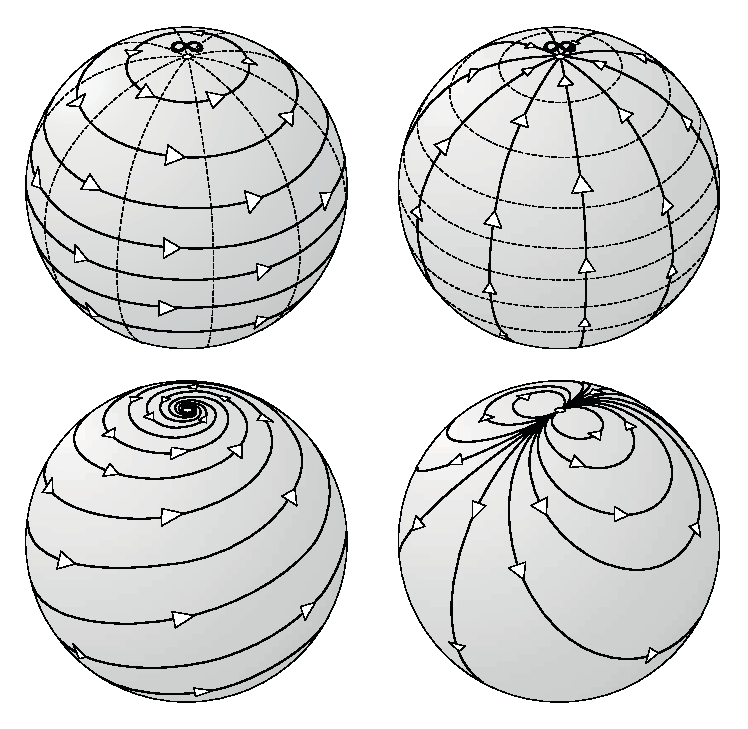
\includegraphics{media/tikz/mobius_transforms_needham.eps}};
    \node at (-3.1, 6.3) {\textbf{Elliptic}};
    \node at (3.2, 6.3) {\textbf{Hyperbolic}};
    \node at (-3.3, -6.3) {\textbf{Loxodromic}};
    \node at (3.3, -6.3) {\textbf{Parabolic}};
    \draw (-6.5, 0) -- (6.5, 0);
    \draw (0, -6.5) -- (0, 6.5);
\end{tikzpicture}

    \caption{Overview of the four classes of Möbius transform and their typical action on the Riemann sphere. The curves shown on the Riemann sphere are the \emph{invariant curves} of the transformation, i.e. these curves as a whole remain invariant under the transformation. Clearly, the elliptic, hyperbolic and loxodromic transformations have the North and South pole, or \(\infty\) and 0 as fixed points, whereas the parabolic transformation only has a single fixed point at the North pole. The loxodromic transformations borrow their name from loxodromes, which are spiral-like trajectories on the Earth with constant bearing --- a ship that taking a loxodromic path would maintain a constant angle with respect to true North. Illustration reprinted from \citet[p. 78]{Needham2021}.}
    \label{fig:riemann_transforms}
\end{figure}

\Cref{tab:moebiusclasses} provides an overview of the five Möbius classes, together with the values for the matrix trace, the multiplier and the Jordan form. Finally, \cref{fig:riemann_transforms} visualizes the effect of each of the transform classes on points on the Riemann sphere. Elliptic transforms push points along circles of constant latitude, while hyperbolic transforms move points orthogonally, along the meridians of the Riemann sphere. Loxodromic transforms are compositions of hyperbolic and elliptic transforms, the associated trajectories therefore look like spirals; incorporating both a North-South and an East-West movement.
\begin{table}
    \caption{Overview of the five classes of Möbius transforms and the corresponding values for the trace squared of the matrix (\(\trace{M} = a + d\)), the multiplier of the transform and the Jordan form.}
    \label{tab:moebiusclasses}
    \centering
    \begin{tabular}{lcccc}
        \toprule
        \textbf{Class} & \textbf{Multiplier} & 
        \(\qty(a + d)^2\) & \textbf{Jordan form} & \textbf{Parent class} \\
        \midrule
        Circular    & \(\qty{-1}\)  &  \([0, 4)\) & 
                      \(\mqty(0 & -1 \\ 1 & 0)\) & Elliptic   \\[0.8cm]
        Elliptic    & \(\qty{k \in \complex \mid \abs{k} = 1, k \neq 1}\)   &  \([0, 4)\) &
                      \(\mqty(\ec^{\theta\ii/2} & 0 \\ 0 & \ec^{-\theta\ii/2})\) & ---  \\[0.8cm]
        Parabolic   & \(\{1\}\)  &  \(\qty{4}\)  & 
                      \(\mqty(1 & b \\ 0 & 1)\) & --- \\[0.8cm]
        Hyperbolic  & \(\real^+_{0}\setminus\qty{1}\) & \((4, +\infty)\)& 
                      \(\mqty(\ec^{\zeta/2} & 0 \\ 0 & \ec^{-\zeta/2})\) & Loxodromic \\[0.8cm]
        Loxodromic  & \(\qty{k \in \complex \mid \abs{k} \neq 1 }\)  & \(\complex\setminus[0, 4]\) &
                      \(\mqty(k & 0 \\ 0 & k^{-1})\) & --- \\[0.4cm]
        \bottomrule
    \end{tabular}
\end{table}

\section{Subgroups}
Apart from the classification considered in the preceding chapter, there are also several subgroups of the Möbius group that can be distinguished. It is compelling to observe that each of these subgroups can each be identified with one of the `geometry types' that were considered in \cref{chap:hyperbolic_geometry}: those of positive (spherical), zero (Euclidean) and negative (hyperbolic) geometry. For every geometry type, a specific subgroup of the Möbius group will play the role of the direct isometry group in a particular `map' \cite{Needham2021}.

\subsection{Euclidean geometry}
The direct isometries in the Euclidean plane consist simply of translations and rotations. Clearly, a rotation in the complex plane (around the origin) can be represented simply by \(z \mapsto e^{\ii \theta}\), while a translation is \(z \mapsto z + b\) with \(b \in \complex\). Hence, the entire direct isometry group of the Euclidean plane is given by
    \[ \mathfrak{E}(z) = e^{\ii\theta} + b. \]
This group is also called the Euclidean group of dimension two.
\subsection{Spherical geometry}
One of the most prevalent applications of group theory is are the representation of rotations in three-dimensional Euclidean space. Of course, the group associated with these rotations is the special orthogonal group \(\sogroup\). This group is diffeomorphic to the three-dimensional real projective space \(\mathbb{RP}^3\) (intuitively, this space consists of three `directions'). The rotations in \(\real^3\) can also be parameterized by \emph{unit quaternions} (also called \emph{versors}): these represent points on the 3-sphere \(\sphere{3}\). The difference between the 3-sphere and the real projective space is that the latter identifies the \emph{antipodal} parts that are present on the sphere. As such, any rotation in \(\real^3\) corresponds precisely to two points on the 3-sphere (or two unit quaternions) --- the group of unit quaternions therefore is a double cover of \sogroup. 

Quaternions can also be represented as complex matrices: \cite{Stillwell2008}
\[ q = \quat{m}{n}{o}{p} \in \quaternions \corresponds Q = \mqty(m + \ii p & -n - \ii o\\n - \ii o & m - \ii p),\]
which is a general represention of a \(2\times 2\) \emph{unitary}\footnote{A unitary matrix is a matrix whose inverse is its conjugate transpose --- it is the complex counterpart of orthogonal matrices.} matrix. Likewise, the unit quaternions then translate to matrices of the above type with an additional restriction: they must have a determinant of 1: these matrices are members of the \emph{special unitary group} \sugroup{2}. As such, the group of unit quaternions is isomorphic to the \sugroup{2} which is therefore also a double cover of \sogroup.

Since the members of \sugroup{2} can be identified with a Möbius transform (inspection of the matrix above makes this immediately apparent), a specific subgroup of \moebiusgroup can be used to represent the rotations in \(\real^3\) --- recall that every normalized Möbius transform also corresponds to two matrices, differing by a factor -1. Observing the matrix above, one can see that the entries on the main diagonal are each others' conjugate, while the entries on the antidiagonal are conjugate opposite. Therefore, the general expression of a rotation of the Riemann sphere as a Möbius transform can be written as: \cite{Needham2021}
\[\mathfrak{S} = \frac{az + b}{-b\bar{z}+\bar{a}}\quad\text{where } \abs{a}^2 + \abs{b}^2 = 1; \]
the latter equivalent then enforces that \(\det Q = 1\). There are always two quaternions representing the same rotation; they are antipodal and differ by a factor of \(-1\). As a result, there are two possibilities for \(Q\) as well, again identical but with opposite entries. Recall that the same applies to the matrix representations of Möbius transforms: as such, the ambiguities are eliminated, and the group of transforms of type \(\mathfrak{S}\) is isomorphic to \sogroup. In the complex plane, these tranformations represent the isometries of spherical geometry in the stereographic map \cite{Needham1997}. 

\index{versor}
\index{quaternion}

\subsection{Hyperbolic geometry}
The normalized transforms with real entries
\[\mathfrak{H}(z) = \frac{az + b}{cz + d}\qquad a, b, c, d \in \real \quad ad - bc = 1;\]
are the isometries of the Poincaré half plane \cite{Needham2021}. [...]

\section{Relation with special linear group}
Another classic Lie group is the special linear group \slgroup{n}{\field}, which are the volume-preserving transformations on a vector space --- this property turns out to be quite important. The special linear group over the complex numbers (2-dimensional) \slgroup{2}{\complex} can be represented as the group of all the complex \(2\times2\) matrices with unit determinant. It has been mentioned previously that any such matrix coincides with a Möbius transform, albeit surjectively: for every Möbius transform, there are two such matrices. As such, \slgroup{2}{\complex} is a \emph{double cover} of \moebiusgroup.

Arguably more interesting than \slgroup{2}{\complex} is the special linear group over the reals \slgroup{2}{\real}, i.e. every invertible \(2 \times 2\) matrix with real entries and a unit determinant; they form a subgroup of \slgroup{2}{\complex} as well. It has been mentioned before that the for the normalized Möbius transforms, the eigenvalues should be complex inverses of each other. For matrices with real entries, the eigenvalues are either both real or complex conjugates of each other. When not on the real axis, the only way eigenvalues can be complex inverses and complex conjugate is to be located on the unit circle. As can be seen on \cref{fig:multiplier_regions}, that means that the matrices with real entries contain exactly the hyperbolic (both real), elliptic (unit circle) and parabolic classes. The remaining part are the loxodromic transforms which have a nonreal trace [CHECK].


\subsection{Relation to flow maps of linear ODE's}

\section{Relation with Lorentz group}

\section{Chapter summary}

\begin{figure}
    

\end{figure}



\chapter{Research proposal}
\label{chap:proposal}
\citet{Mankiw2017} define three roles of money in society:
\begin{enumerate}[itemsep=0.2ex,parsep=0ex,label=(\roman*),topsep=0.2ex]
    \item a \emph{medium of exchange}; i.e. a universal means of exchanging goods and services without the necessity for bartering, 
    \item a \emph{unit of account}; a measuring stick to compare different goods by means of their prices;
    \item a \emph{store of value}, which allows translating present earnings to the future.
\end{enumerate}
A sound framework in economic engineering should be able to assign  a precise interpretation to each of these roles. The medium of exchange is encapsulated in the `price' component of the price-quantity phase space that underlies the economic engineering theory. Likewise, the role of money as a unit of account is reflected in the symplectic structure of the economic phase space: as shown in \cref{sec:hamilton_eqs}, the symplectic form (which represents a differential amount of revenue `traced out' in the phase plane) provides an isomorphism between the covariant and contravariant tensor components. However, this does not cover other notions to which the unit of account may apply, such as the substitution effect; so this interpretation may have to be refined. Finally, the role of money as a store of value has been the most problematic in the past because of (i) its inherent temporal aspect and (ii) the idea that earnings (which are analogous to energy) are converted to either a generalized momentum or a generalized position. This `store of value' problem is most apparent when one tries to model investments of any kind, such as stocks, bonds, derivatives, debt, and equity, etc.

It has been shown in the past that financial (sub)systems (that is, economic systems that include the market dynamics of investments) are an essential component of the larger economic system, as demonstrated by \citet{Kruimer2021}, \citet{Vos2019} and \citet{VanArdenne2020}. In past economic engineering research, two prevalent interpretations have been assigned to financial instruments: action-angle coordinates (cf. \cref{chap:ee}) and the rotational analogy (cf. \cref{chap:finance_rotation}). However, both problems present some crucial issues:
\begin{itemize}
    \item The \textbf{action-angle approach} is based on a special canonical transformation of the phase space coordinates that are used in physics to facilitate the integration of complex systems or make statements about their periodicity. Their application on financial systems is based on the fact that they consist of dimensionless angle coordinates (`return') and action coordinates with units of money (`investment'). However, this seems to be an ad hoc solution, since the formal applicability of action-angle coordinates is very precise; they can only be used for conservative and conditionally periodic systems \cite{Arnold1989}. For this reason, the angle coordinates have a constant `angular velocity': clearly, this is not at all representative of the return rate in economics. Likewise, the action coordinates are supposed to be functions of first integrals of the system (and therefore time-invariant); again, this does seem unlikely for the investments in dynamic economic systems. 
    
    This approach may have worked in an applied modeling context by producing the correct dynamics, but the direct correspondence with investments and return evidently does not hold up to more rigorous standards. This does not mean that there is no place for action-angle coordinates in economic engineering whatsoever, take for example the business cycle analogy that is proposed in \cref{sec:hamilton_eqs}.
\item The issues with the \textbf{rotational analogy} are more subtle, but they have far-reaching ramifications nevertheless. As \cref{sec:rotational_analogy} already presented, there is definitely something to say for the `rotational' part, i.e. viewing interest as a hyperbolic rotation --- this is the entire point of \cref{chap:finance_rotation}. Basically, one can argue that the kinematics hold, but the application of the dynamics shows some shortcomings: for example, the difference between the arm and the angular momentum, which both have identical units, the interpretation of rotational kinetic energy. Furthermore, duration has been proposed as being equivalent to the mass moment of inertia, but does this does not cover the full character of financial instruments; beside the fact that duration is now considered to be a valuation concept that belongs in frequency-domain analysis \cite{Krabbenborg2021,Kruimer2021}. In the past, the rotational analogy has been used for modeling in a similar fashion as the action-angle coordinates, simply by defining the amount invested and the return as conjugate variables in the same way as `traditional' prices and quantities are related in economic engineering. In that sense, the \emph{application} of the rotational analogy is roughly equivalent to the application of action-angle coordinates.
\end{itemize}
Given the importance of financial systems, a solution to these problems will benefit economic engineering research and its applicability to real situations. It can be observed that the quest for suitable analogies to money and financial instruments is hampered by the `unit problem'; that is, many quantities are expressed in terms of money while they play a very different role: for example, the distinction between money as energy (income) and as a quantity or momentum, or the difference between capital and yield. Whereas dimensional analysis has been an instructive practice in other applications of economic engineering, employing it carelessly in this situation quickly leads to inconsistencies. For example, the rotational analogy requires the continuous transformation between direct earnings on interest to capital; from a fundamental standpoint, these may correspond to quantities of a different nature; other types of financial instruments (e.g. stocks) suggest that this process should be `pulled apart', for it conceals the underlying mechanism of reinvestment.

As such, the aim of this research is to return to find the solution of this problem in the fundamentals of economic engineering as they are presented in \cref{chap:ee}, as to formulate a consistent interpretation of financial instruments. These fundamentals consist of the concept of utility as energy and the symplectic structure of the economic phase plane. Because of the unit problem, it is often unclear in finance what has the role of products and prices (or even something else); this will naturally appeal to the usage of canonical coordinate transforms of the regular phase space or a Routhian approach where the Hamiltonian and Lagrangian approach are essentially merged. The idea is to find a mapping between these central concepts and the fundamental theory of interest and utility, in particular the work of Irving Fischer \cite{Fisher1906,Fisher1930}.

Other questions that are to be answered pertain to financial equilibria and conservation principles. For example, the classic mechanical equilibrium (Galilean frame of reference) consists of a mass moving at a constant velocity; in economic engineering, this would be a demander with a constant consumer surplus or a producer with a constant producer surplus; consequently, market prices remain constant over time. This and other conservation laws are governed by Noether's theorem (cf. \cref{ssec:noether}). The crucial link between Noether's theorem and the structure behind the Lagrangian and Hamiltonian utility functions will provide insights that would otherwise be shrouded by the unit problem or the potentially complex differential equation that describes the evolution. Usually, the latter is used to understand the nature of the economic system, but the case is made here that analysis of the Lagrangian and Hamiltonian functions is usually more efficient and instructive.

Although the main goal of this research is to improve the understanding of financial systems, the rigorous methods that will be applied may contribute to economic engineering in general as well. For example, the application of manifold theory to economic systems, both from the perspective of the configuration manifold and the cotangent bundle or phase space. Until now, the natural structure of these spaces has not been researched in depth. Additionally, Hamiltonian and Lagrangian analysis are usually not deemed suitable for dissipative systems; but \citet{Hutters2020} demonstrated how Hamiltonian systems can be applied to systems with linear damping. Because real economic systems are always dissipative (just like their mechanical counterparts), this method may be applied to financial systems as well.

Finally, the incorporation of the nature of capital in the economic engineering framework can be used to explain heavily debated concepts such as inflation, monetary policy, and banking regulation. For example, there have been disputes in  macroeconomic theory about whether inflation is endogenous (that is, it arises naturally) or exogenous to economic systems. This is one example where conservation principles may prove their value in economic systems.


%========================== Appendices =======================================
\appendix
%
%
% An Appendix
\chapter{Some math}
A topology is a collection of elements from the power set of a given set. Roughly speaking, a topology gives rise to a notion of `neighborhoods', which further allows for the concepts of convergence and continuity to be properly defined on a set.

Definitions from \cite{Lee2000}

\begin{definition}[Inner product]
    An \emph{inner product} on a real vector space $V$ is a function from $V \times V$ to $\real$, denoted by $(\vb{u}, \vb{v}) \mapsto \langle \vb{u}, \vb{v} \rangle$ such that for all $\vb{u}, \vb{v}$ in $V$
    \begin{enumerate}
        \item $\langle \vb{u}, \rangle$ and $\langle, \vb{v}\rangle$ are linear functions from $V$ to $\real$ (bilinearity),
        \item $\langle \vb{u}, \vb{v} \rangle$ = $\langle \vb{u}, \vb{v} \rangle$ (symmetry),
        \item If $\vb{u} \neq 0$, then there is a $\vb{v} \neq 0$ such that $\rangle \vb{u}, \vb{v} \rangle \neq 0$ (nondegeneracy).
    \end{enumerate}
    
\end{definition}

\begin{definition}[Topology]
    A \emph{topology} on a set $X$ is a collection $\mathscr{T}$ of subsets of $X$ called \emph{open sets}, satisfying the following properties:
    \begin{enumerate}[label=\roman*]
        \item $X$ and $\varnothing$ are elements of $\mathscr{T}$.
        \item $\mathscr{T}$ is closed under finite intersections; if $U_1,\ldots,U_n \in \mathscr{T}$, then their intersection $U_1 \cap \ldots \cap U_n$ is in $\mathscr{T}$.
            \item $\mathscr{T}$ is closed under arbitrary unions: if $U_{\alpha \in A}$ is any (finite or infinite) collection of elements of $\mathscr{T}$, then their union $\displaystyle\bigcup_{\alpha \in A}  U_\alpha$ is in $\mathscr{T}$.
    \end{enumerate}
\end{definition}
\begin{definition}[Homeomorphism]
    If $X$ and $Y$ are topological spaces, a \emph{homeomorphism} from $X$ to $Y$ is defined to be a continuous bijective map $\varphi: X\to Y$ with continuous inverse. If there exists a homeomorphism between $X$ and $Y$, they are called homeomorphic or topologically equivalent.
\end{definition}

%%
% Another appendix chapter
\chapter{Differential geometry and topology}



%========================== Back matter ======================================

\backmatter
%
% Bibliography
\printbib{library}
%
%% SYMBOL TERMINOLOGY
% \gsymb{} Greek symbols γ
% \lsymb{} Letter symbols H(s)
% \supers{} Superscript symbols only printed in the List of Symbols
% \subs{} Subscript symbols only printed in the List of Symbols
% \others{} Other symbols only printed in the List of Symbols

% Glossary
\chapter{Glossary} %
%
\printacronyms
\begin{acronym}[\hspace{0.8in}] % 0.8in is also used by the nomenclature
    \acro{IRR}{Internal Rate of Return}
    \acro{NPV}{Net Present Value}
	
\end{acronym}%


% Nomenclature
\printnomencl%
% test
% Index
\cleardoublepage
\printindex
%%%%%

\end{document}
